%%%%%%%%%%%%%%%%%%%%%%%%%%%%%%%%%%%%%%%%%%%%%%%%%%%%%%%%%%%%%%%%%%%%%%%%%%%%%%%%%%
\begin{frame}[fragile]\frametitle{}
\begin{center}
{\Large Background}\\

{till word2vec}

\end{center}
\end{frame}



%%%%%%%%%%%%%%%%%%%%%%%%%%%%%%%%%%%%%%%%%%%%%%%%%%%%%%%%%%%
\begin{frame}[fragile]\frametitle{How do we represent the meaning of a word?}
Definition: meaning (Webster dictionary)

\begin{itemize}
\item the idea that is represented by a word, phrase, etc.
\item the idea that a person wants to express by using  words, signs, etc.
\item the idea that is expressed in a work of writing, art, etc.  
\end{itemize}

Commonest linguistic way of thinking of meaning:

\begin{center}
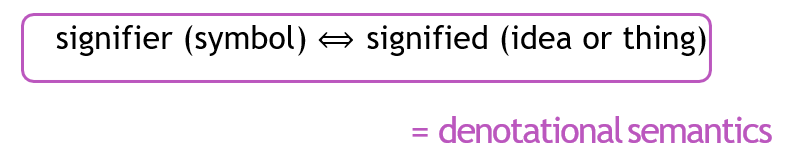
\includegraphics[width=0.6\linewidth,keepaspectratio]{bert2}
\end{center}		  

{\tiny (Ref: CS224n: Natural Language Processing with Deep Learning - Christopher Manning)}

\end{frame}


%%%%%%%%%%%%%%%%%%%%%%%%%%%%%%%%%%%%%%%%%%%%%%%%%%%%%%%%%%%
\begin{frame}[fragile]\frametitle{How do we have usable meaning in a computer?}


\begin{center}
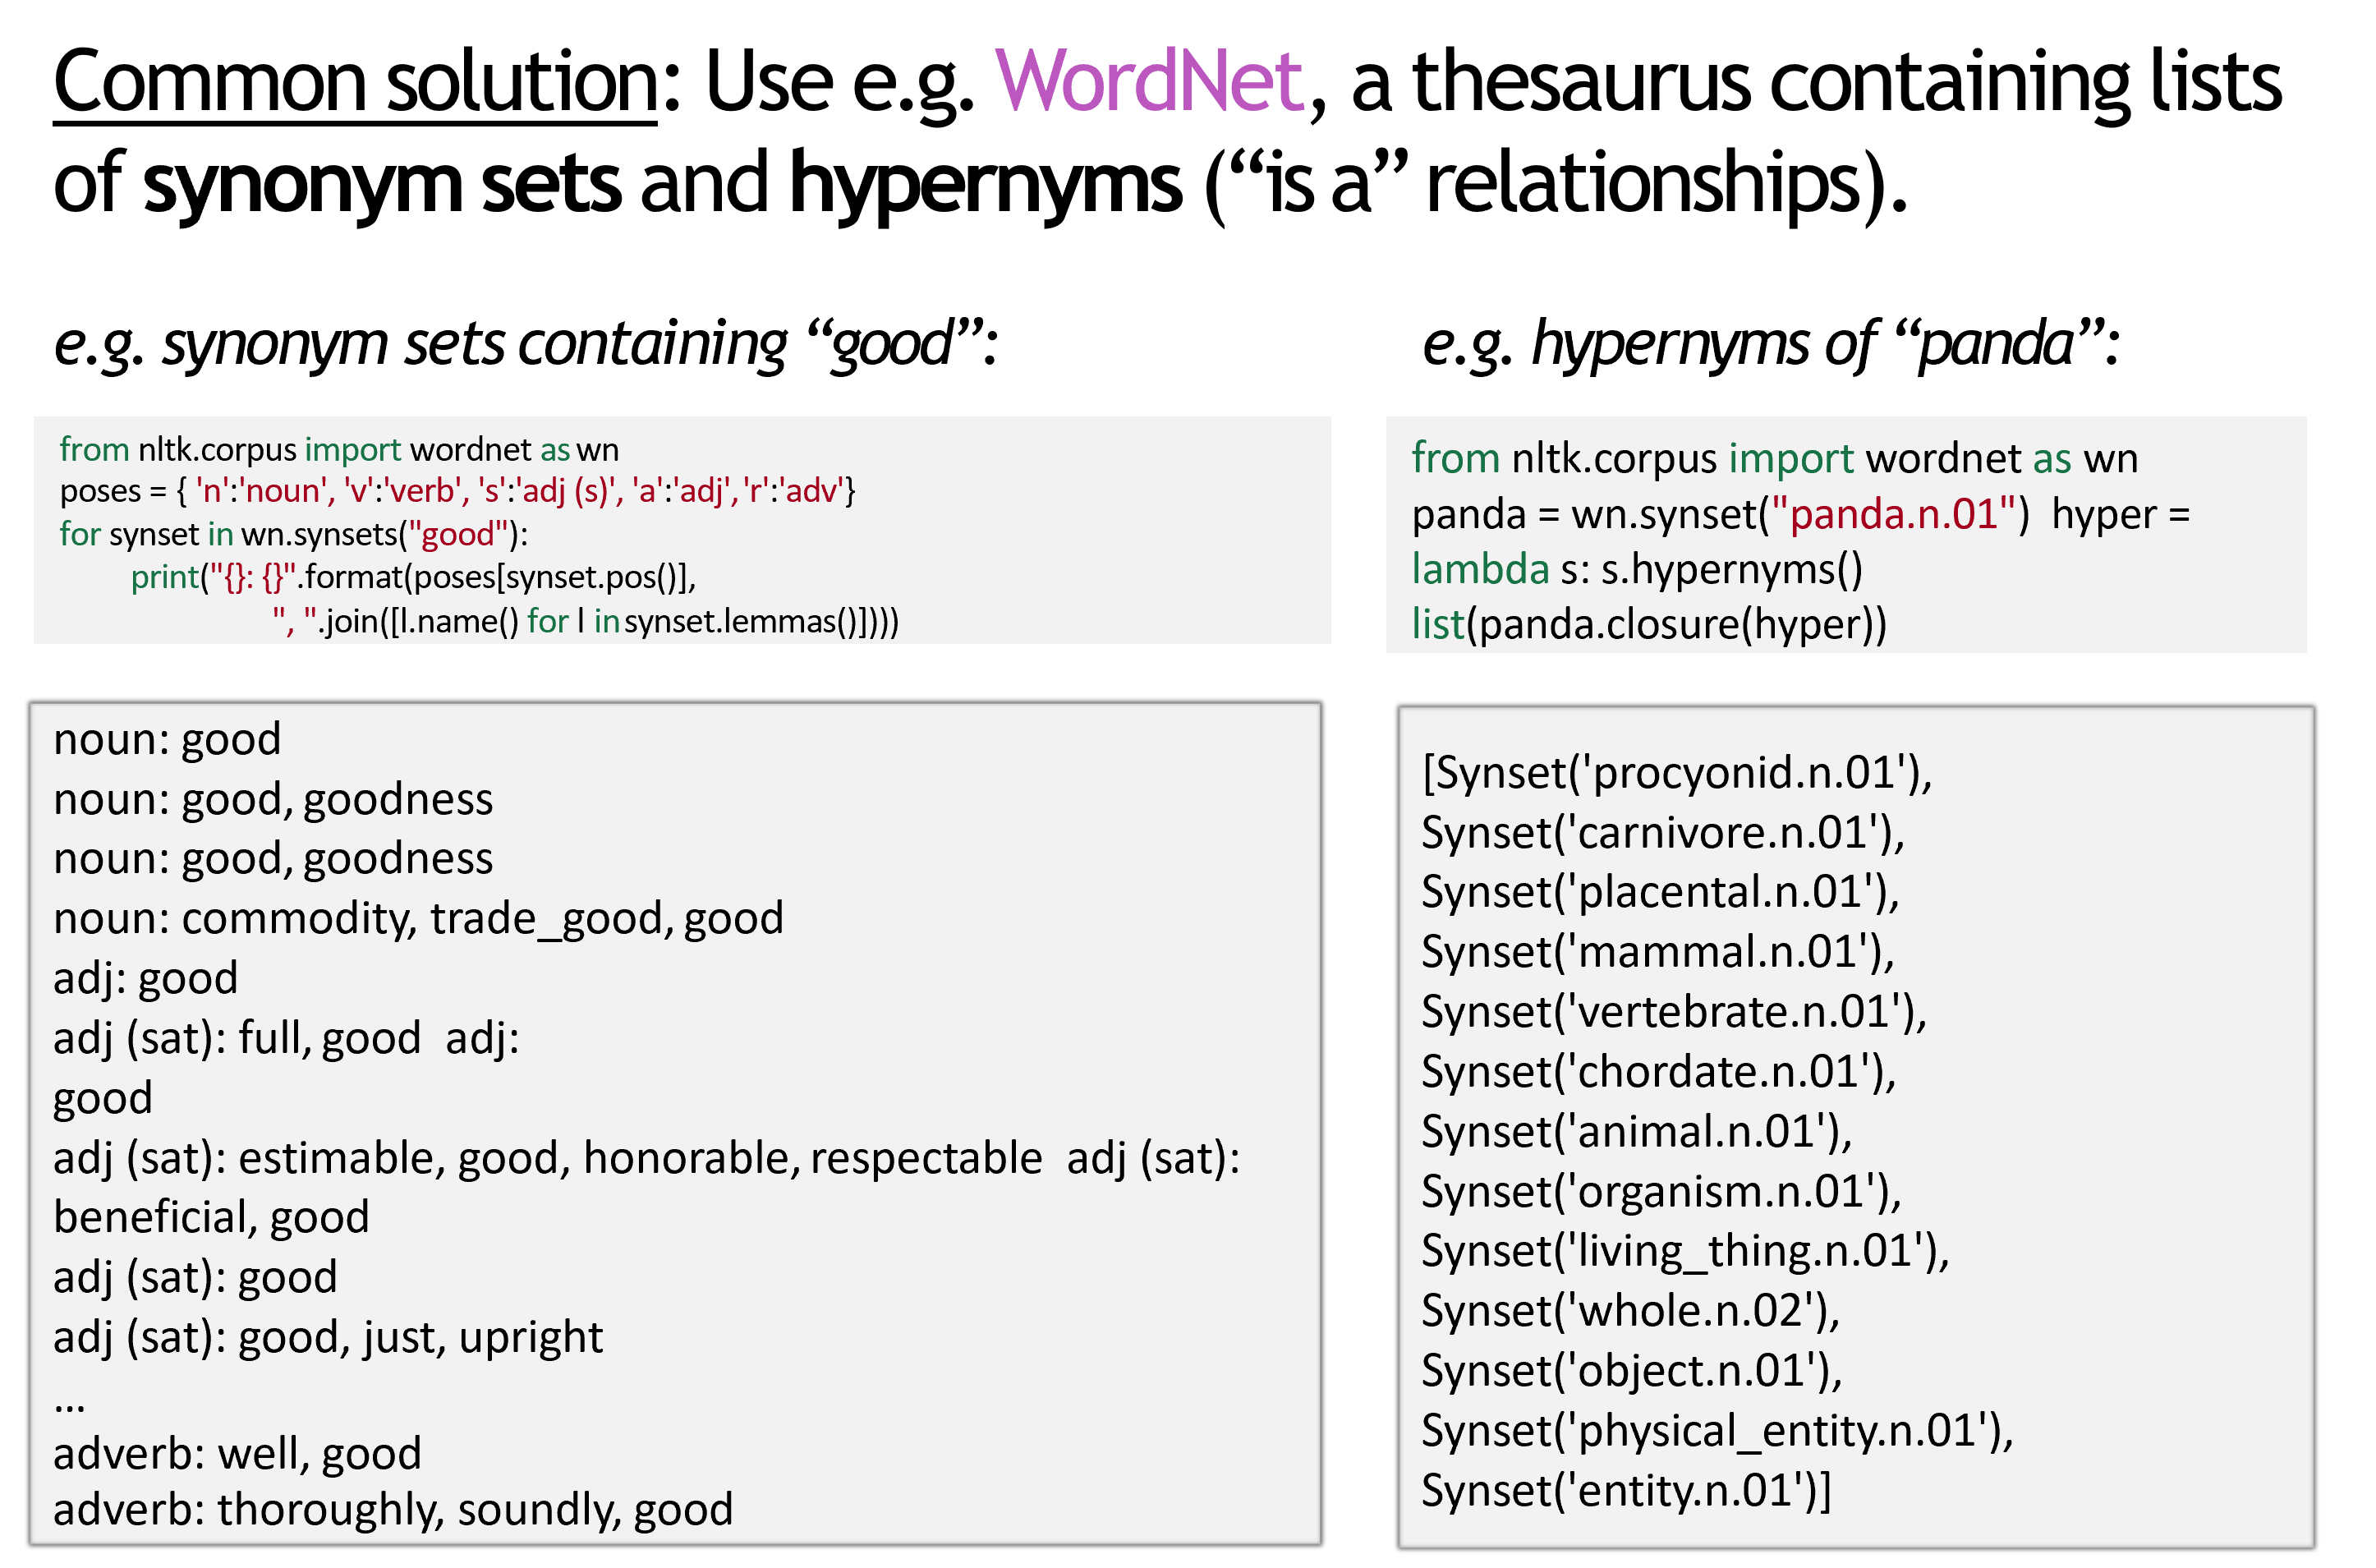
\includegraphics[width=\linewidth,keepaspectratio]{bert3}
\end{center}		  

{\tiny (Ref: CS224n: Natural Language Processing with Deep Learning - Christopher Manning)}

\end{frame}

%%%%%%%%%%%%%%%%%%%%%%%%%%%%%%%%%%%%%%%%%%%%%%%%%%%%%%%%%%%
\begin{frame}[fragile]\frametitle{Problems with resources like WordNet}


\begin{itemize}
\item Great as a resource but missing nuance: e.g. ``proficient'' is listed as a synonym for ``good''.  This is only correct in some contexts.
\item Missing new meanings of words: e.g., wicked, badass, nifty, wizard, genius, ninja, bombest. Impossible to keep up-to-date!
\item Subjective
\item Requires human labor to create and adapt
\item Can't compute accurate word similarity 
\end{itemize}

{\tiny (Ref: CS224n: Natural Language Processing with Deep Learning - Christopher Manning)}

\end{frame}

%%%%%%%%%%%%%%%%%%%%%%%%%%%%%%%%%%%%%%%%%%%%%%%%%%%%%%%%%%%
\begin{frame}[fragile]\frametitle{Representing words as discrete symbols}


\begin{center}
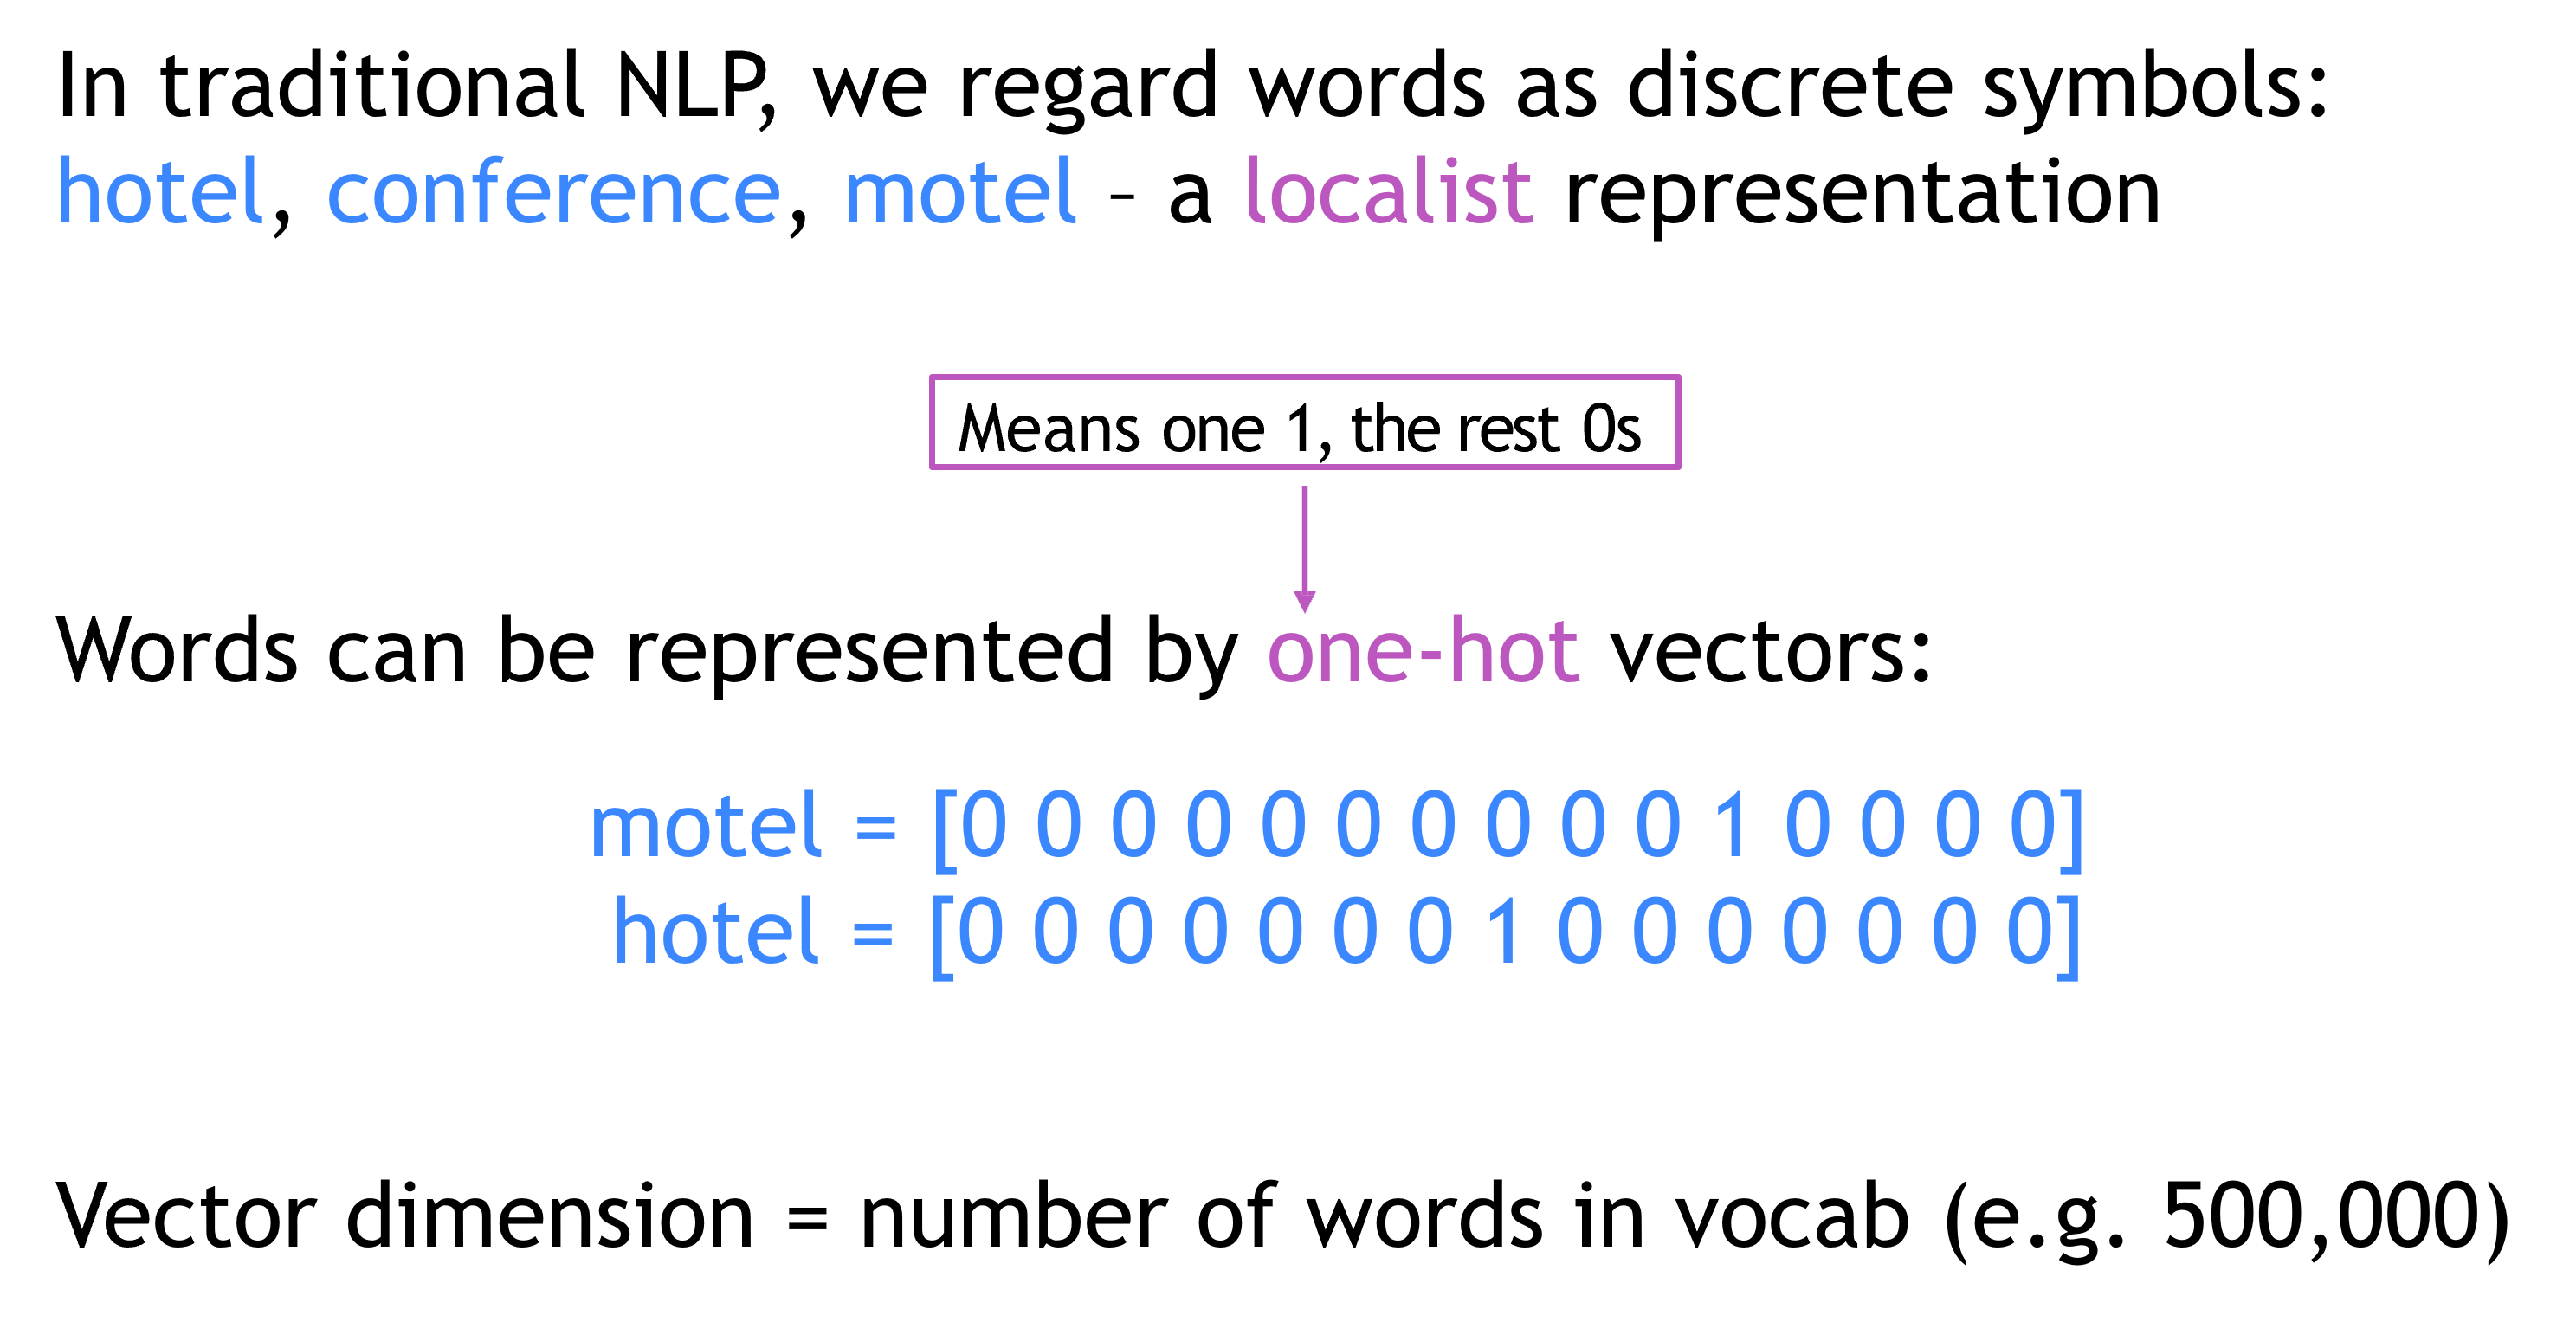
\includegraphics[width=\linewidth,keepaspectratio]{bert4}
\end{center}		  


{\tiny (Ref: CS224n: Natural Language Processing with Deep Learning - Christopher Manning)}

\end{frame}

%%%%%%%%%%%%%%%%%%%%%%%%%%%%%%%%%%%%%%%%%%%%%%%%%%%%%%%%%%%
\begin{frame}[fragile]\frametitle{Representing words as discrete symbols}


\begin{center}
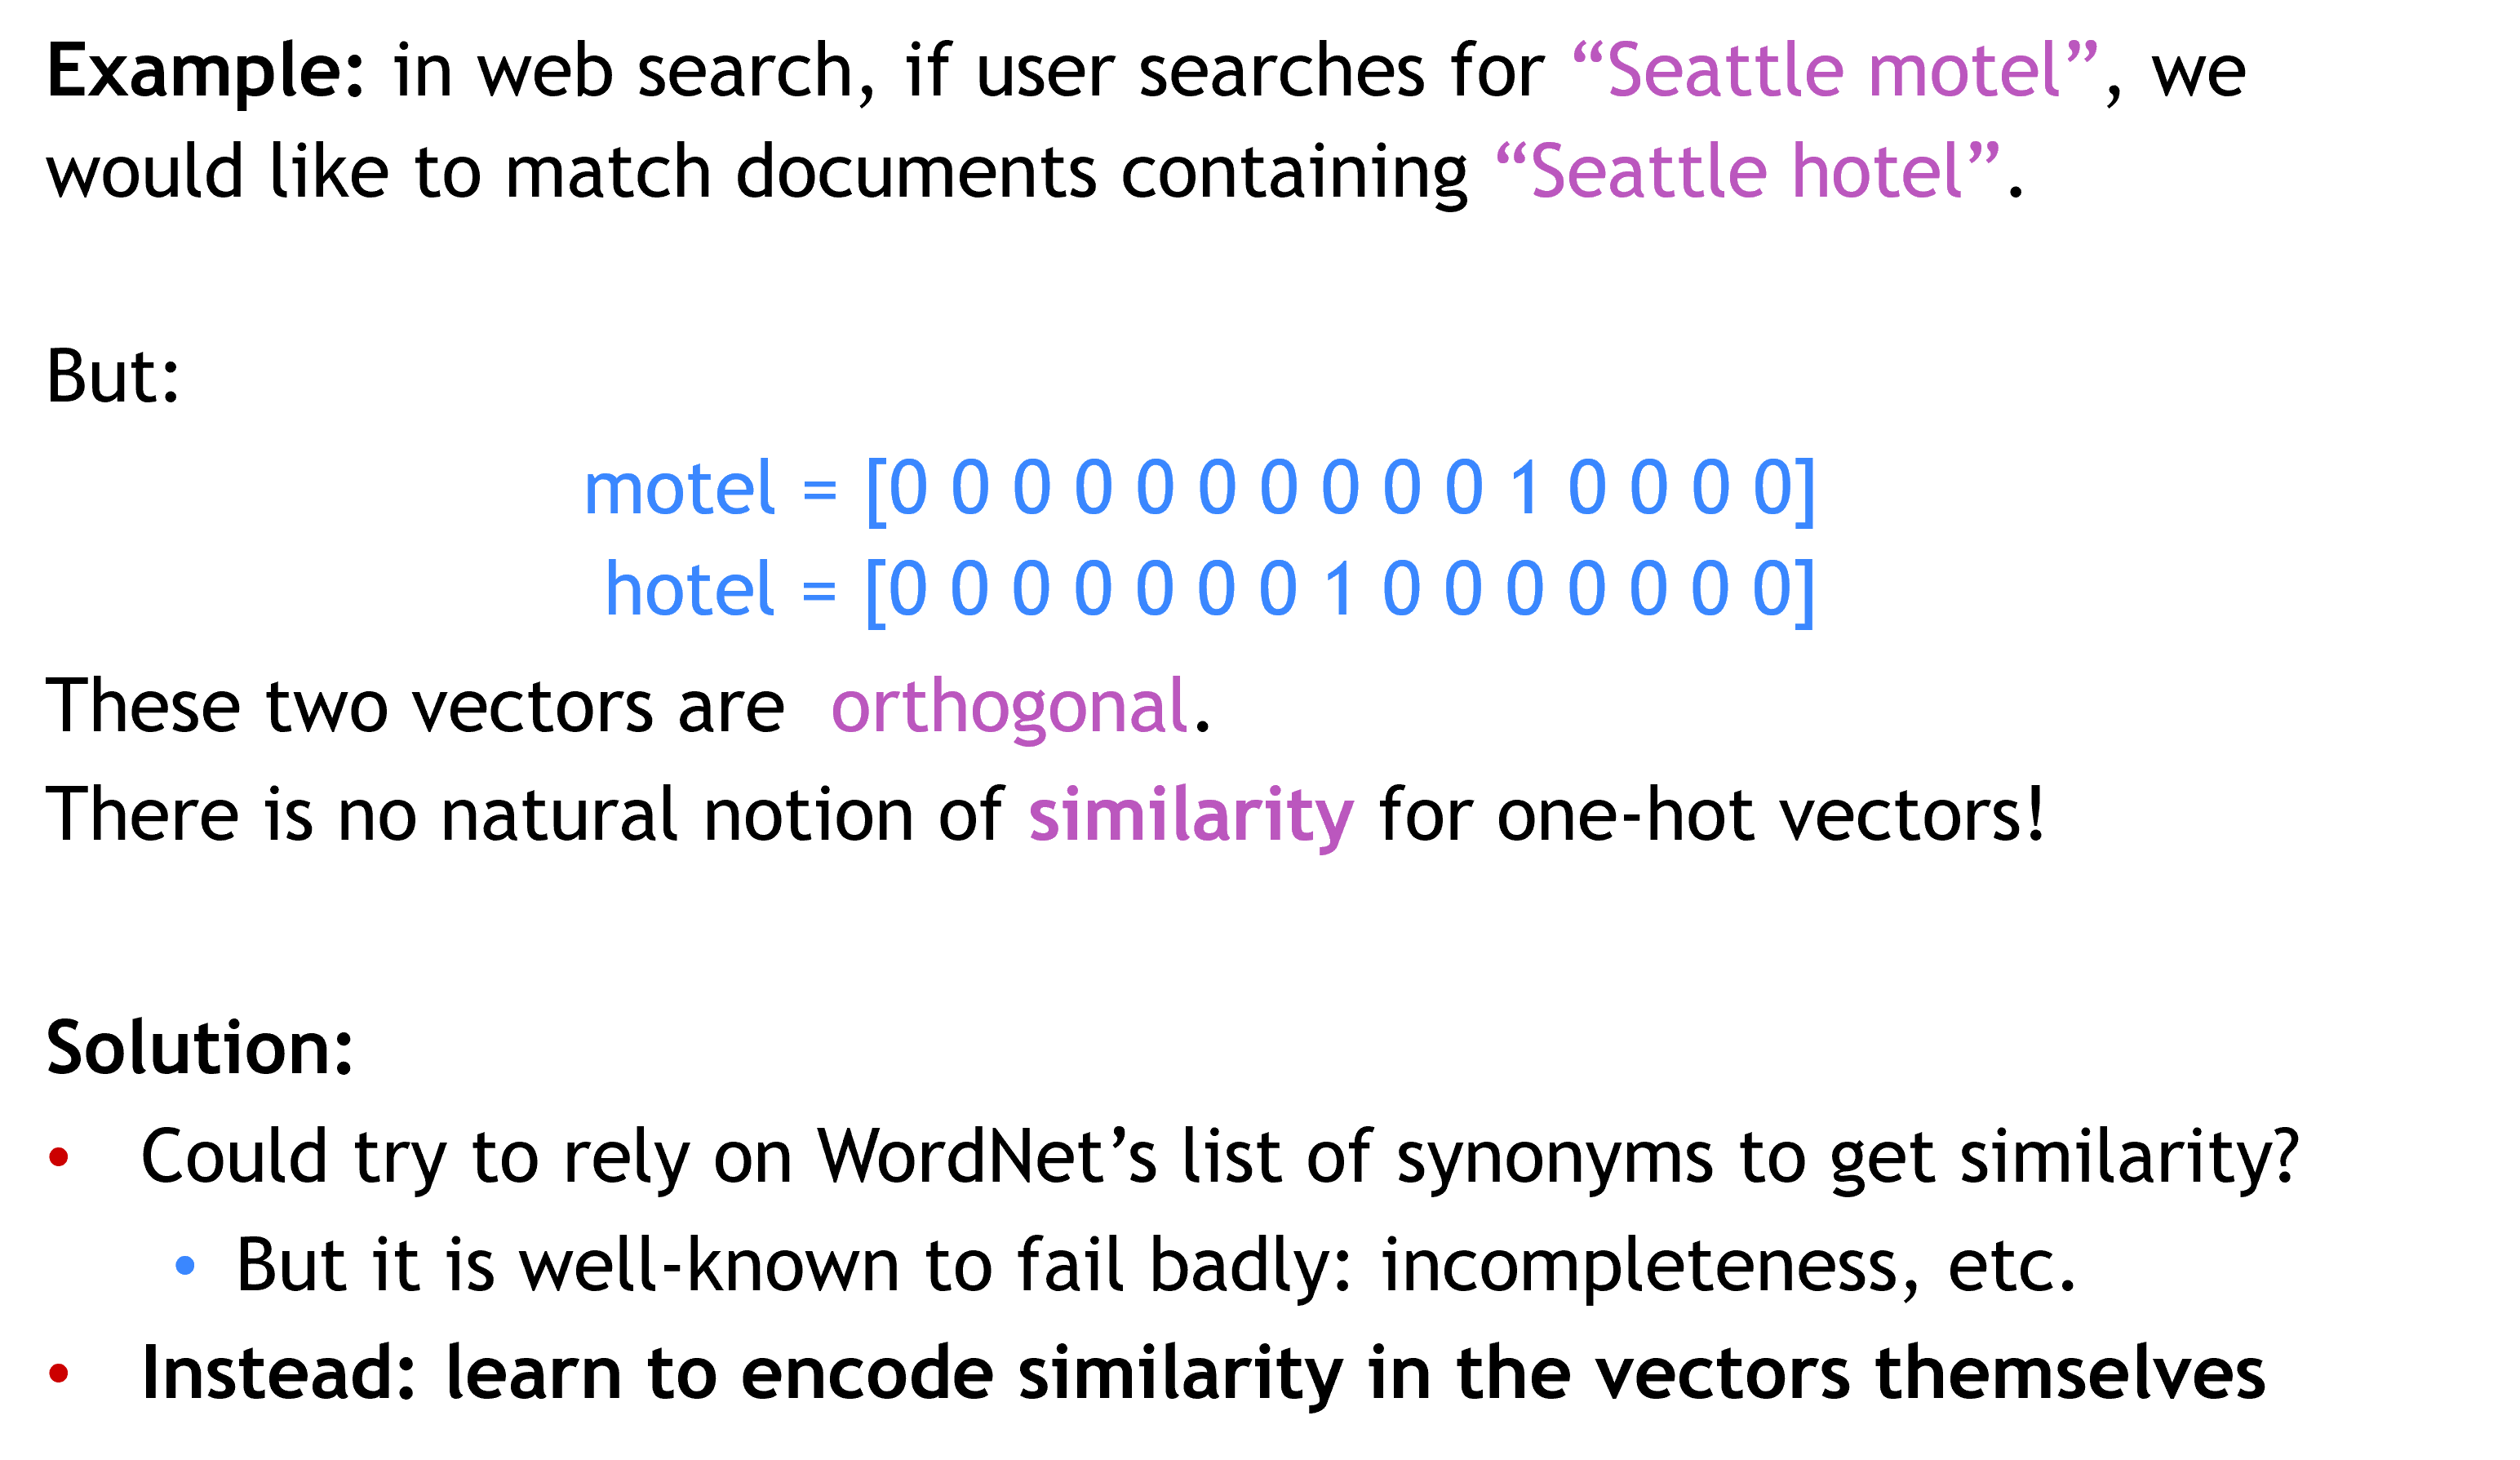
\includegraphics[width=\linewidth,keepaspectratio]{bert5}
\end{center}		  


{\tiny (Ref: CS224n: Natural Language Processing with Deep Learning - Christopher Manning)}

\end{frame}

%%%%%%%%%%%%%%%%%%%%%%%%%%%%%%%%%%%%%%%%%%%%%%%%%%%%%%%%%%%
\begin{frame}[fragile]\frametitle{Representing words by their context}


\begin{center}
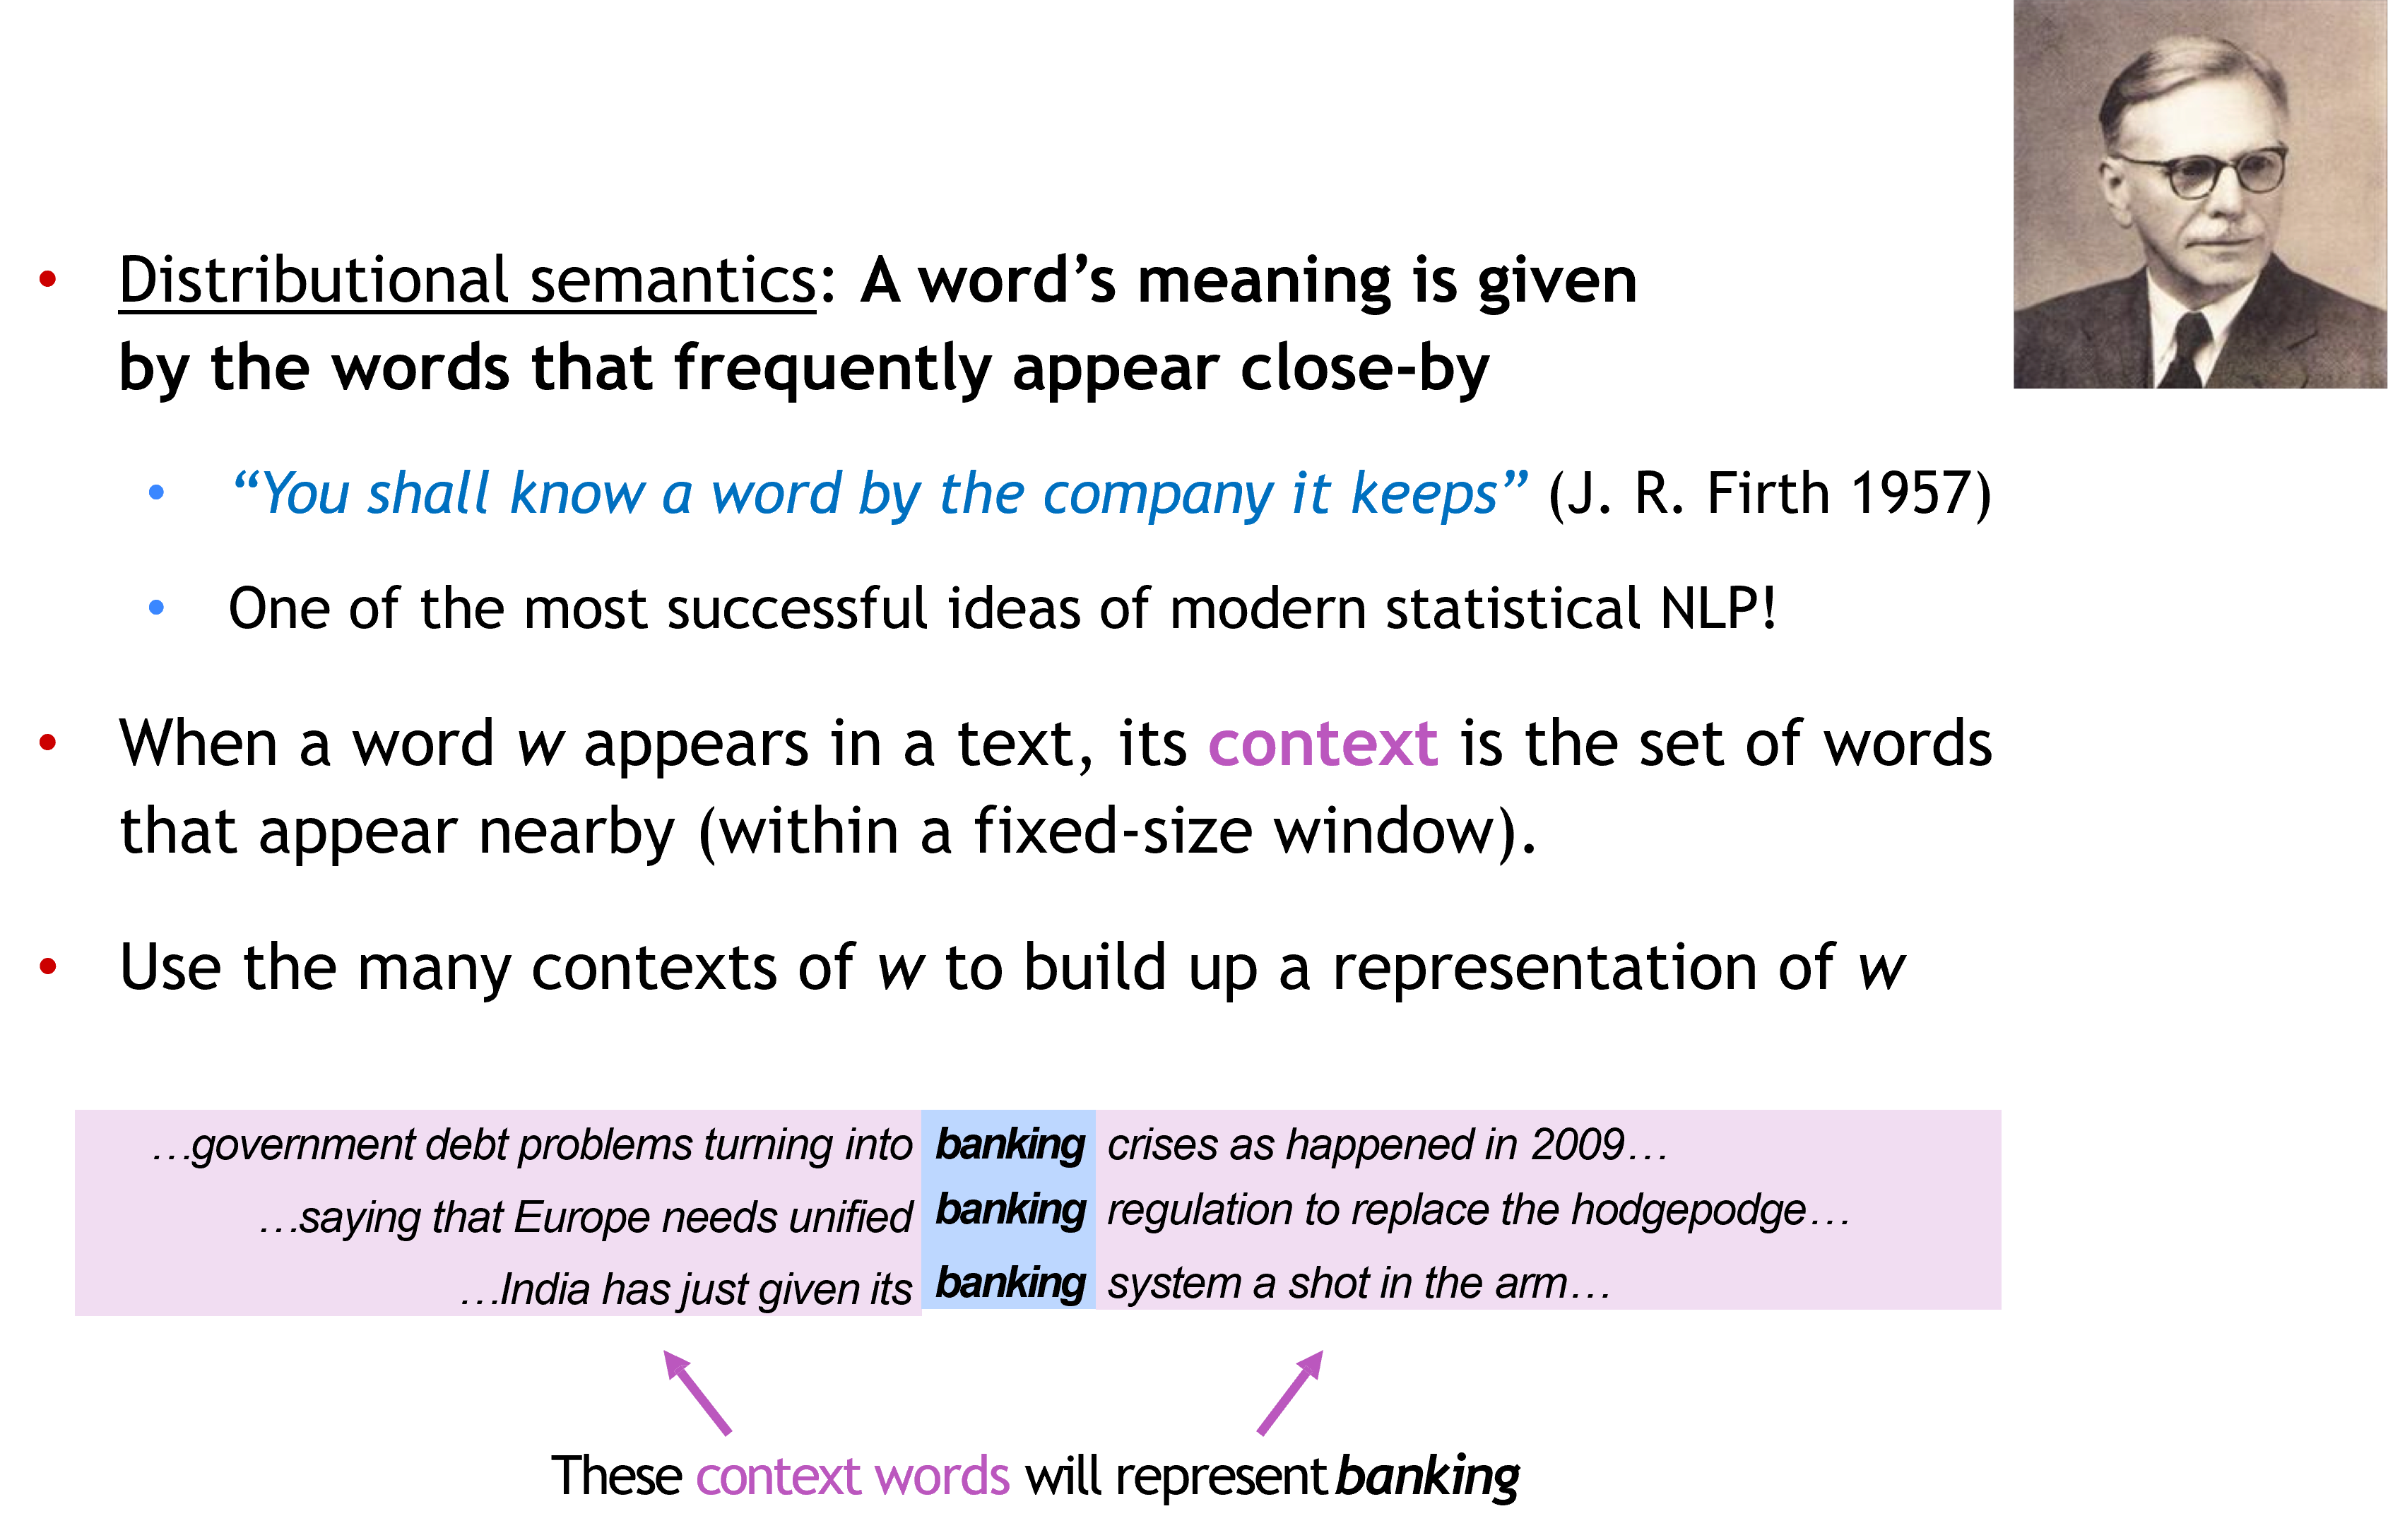
\includegraphics[width=\linewidth,keepaspectratio]{bert6}
\end{center}		  


{\tiny (Ref: CS224n: Natural Language Processing with Deep Learning - Christopher Manning)}

\end{frame}

%%%%%%%%%%%%%%%%%%%%%%%%%%%%%%%%%%%%%%%%%%%%%%%%%%%%%%%%%%%
\begin{frame}[fragile]\frametitle{What can we learn from reconstructing input?}

\begin{center}
Stanford University is located in $---------$	, California.
\end{center}		  

{\tiny (Ref: Language \& Machine Learning - John Hewitt)}
\end{frame}

%%%%%%%%%%%%%%%%%%%%%%%%%%%%%%%%%%%%%%%%%%%%%%%%%%%%%%%%%%%
\begin{frame}[fragile]\frametitle{What can we learn from reconstructing input?}

\begin{center}
I put $----------$ fork down on the table.
\end{center}		  

{\tiny (Ref: Language \& Machine Learning - John Hewitt)}
\end{frame}

%%%%%%%%%%%%%%%%%%%%%%%%%%%%%%%%%%%%%%%%%%%%%%%%%%%%%%%%%%%
\begin{frame}[fragile]\frametitle{What can we learn from reconstructing input?}

\begin{center}
The woman walked across the street, \\ checking for traffic over $----------$ shoulder.
\end{center}		  

{\tiny (Ref: Language \& Machine Learning - John Hewitt)}
\end{frame}

%%%%%%%%%%%%%%%%%%%%%%%%%%%%%%%%%%%%%%%%%%%%%%%%%%%%%%%%%%%
\begin{frame}[fragile]\frametitle{What can we learn from reconstructing input?}

\begin{center}
I went to the ocean to see the fish, turtles, seals, and $----------$.
\end{center}		  

{\tiny (Ref: Language \& Machine Learning - John Hewitt)}
\end{frame}

%%%%%%%%%%%%%%%%%%%%%%%%%%%%%%%%%%%%%%%%%%%%%%%%%%%%%%%%%%%
\begin{frame}[fragile]\frametitle{What can we learn from reconstructing input?}

\begin{center}
Overall, the value I got from the two hours watching \\ it was the sum total of the popcorn and the drink.\\
The movie was  $----------$.
\end{center}		  

{\tiny (Ref: Language \& Machine Learning - John Hewitt)}
\end{frame}

%%%%%%%%%%%%%%%%%%%%%%%%%%%%%%%%%%%%%%%%%%%%%%%%%%%%%%%%%%%
\begin{frame}[fragile]\frametitle{What can we learn from reconstructing input?}

\begin{center}
Iroh went into the kitchen to make some tea.\\
Standing next to Iroh, Zuko pondered his destiny.\\
Zuko left the  $----------$.
\end{center}		  

{\tiny (Ref: Language \& Machine Learning - John Hewitt)}
\end{frame}

%%%%%%%%%%%%%%%%%%%%%%%%%%%%%%%%%%%%%%%%%%%%%%%%%%%%%%%%%%%
\begin{frame}[fragile]\frametitle{What can we learn from reconstructing input?}

\begin{center}
I was thinking about the sequence that goes  \\ 1, 1, 2, 3, 5, 8, 13, 21,   $----------$.
\end{center}		  

{\tiny (Ref: Language \& Machine Learning - John Hewitt)}
\end{frame}

%%%%%%%%%%%%%%%%%%%%%%%%%%%%%%%%%%%%%%%%%%%%%%%%%%%%%%%%%%%
\begin{frame}[fragile]\frametitle{Word vectors}

We will build a dense vector for each word, chosen so that it is  similar to vectors of words that appear in similar contexts
	  
\begin{center}

\includegraphics[width=0.5\linewidth,keepaspectratio]{bert7}
\end{center}		  
		
Note: word vectors are sometimes called word embeddings or  word representations. They are a distributed representation.

{\tiny (Ref: CS224n: Natural Language Processing with Deep Learning - Christopher Manning)}

\end{frame}

%%%%%%%%%%%%%%%%%%%%%%%%%%%%%%%%%%%%%%%%%%%%%%%%%%%%%%%%%%%
\begin{frame}[fragile]\frametitle{Word meaning as a neural word vector: visualization}

	  
\begin{center}
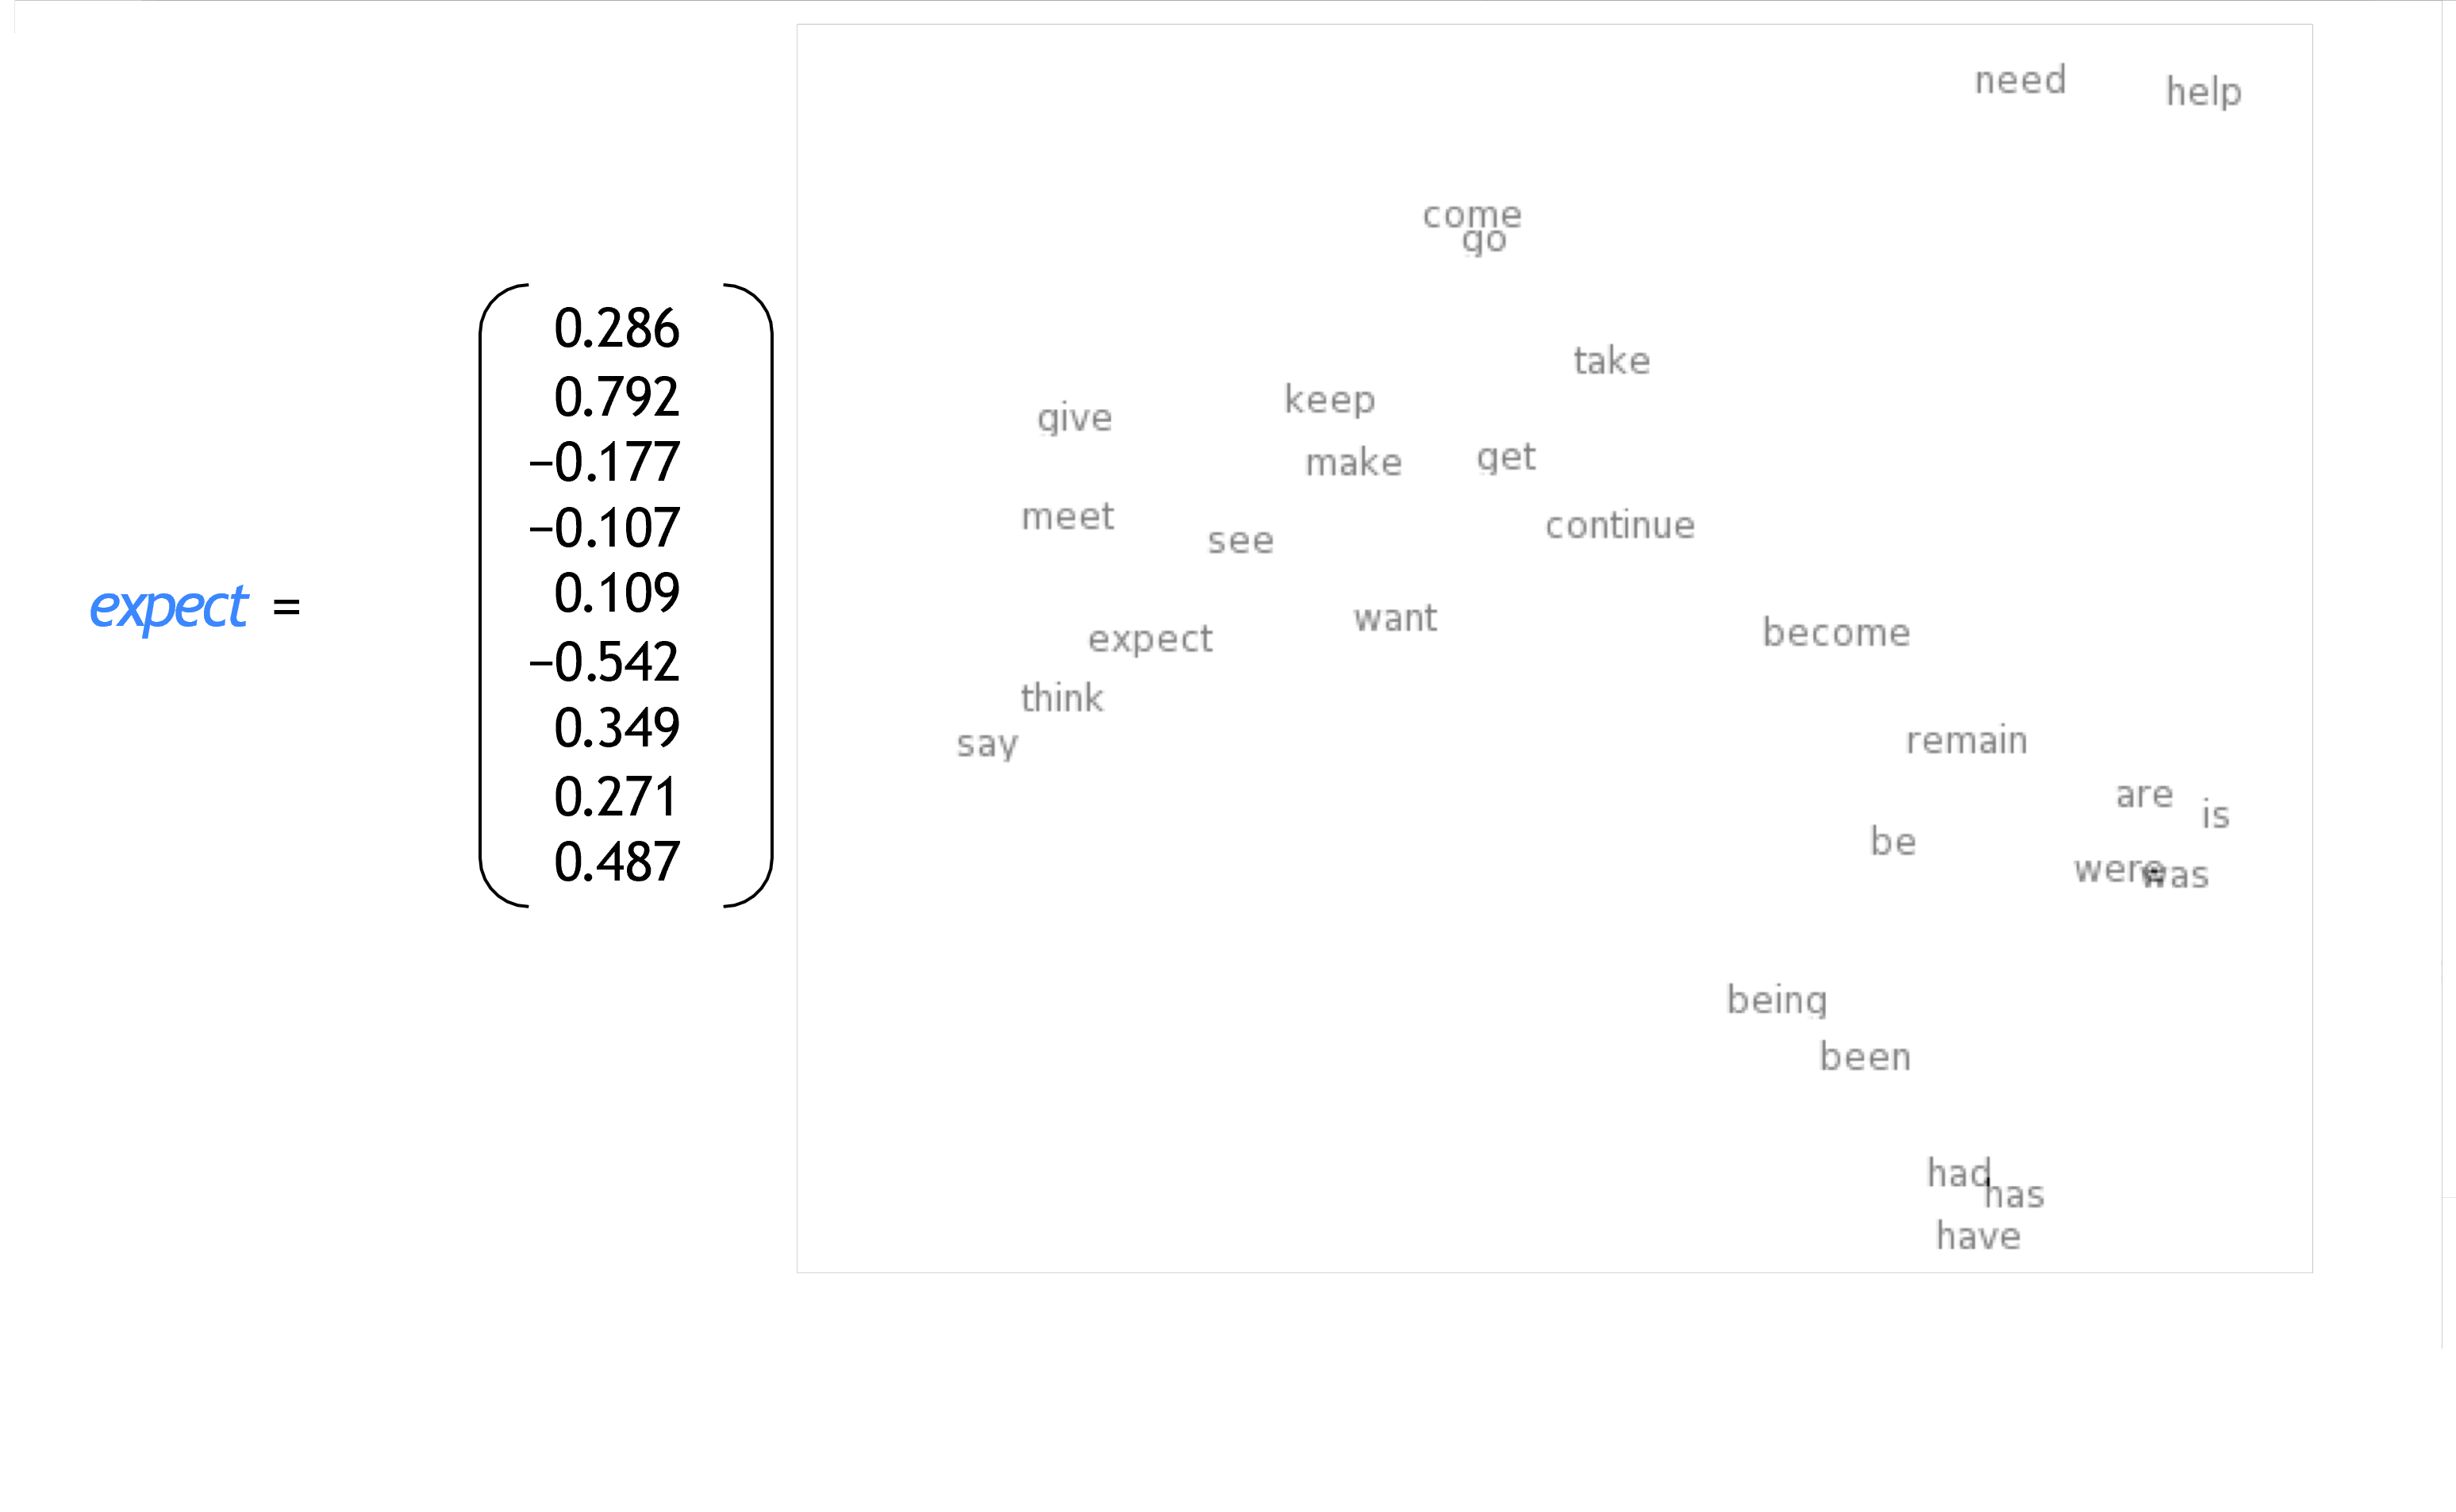
\includegraphics[width=\linewidth,keepaspectratio]{bert8}
\end{center}		  
		

{\tiny (Ref: CS224n: Natural Language Processing with Deep Learning - Christopher Manning)}

\end{frame}

%%%%%%%%%%%%%%%%%%%%%%%%%%%%%%%%%%%%%%%%%%%%%%%%%%%%%%%%%%%
\begin{frame}[fragile]\frametitle{Word2Vec Overview}
Word2vec (Mikolov et al. 2013) is a framework for learning  word vectors

Idea:
\begin{itemize}
\item We have a large corpus of text
\item Every word in a fixed vocabulary is represented by a vector
\item Go through each position t in the text, which has a center word
c and context (“outside”) words o
\item Use the similarity of the word vectors for c and o to calculate  the probability of o given c (or vice versa)
\item Keep adjusting the word vectors to maximize this probability

\end{itemize}

{\tiny (Ref: CS224n: Natural Language Processing with Deep Learning - Christopher Manning)}

\end{frame}



%%%%%%%%%%%%%%%%%%%%%%%%%%%%%%%%%%%%%%%%%%%%%%%%%%%%%%%%%%%%%%%%%%%%%%%%%%%%%%%%%%
\begin{frame}[fragile]\frametitle{}
\begin{center}
{\Large End}
\end{center}
\end{frame}


%%%%%%%%%%%%%%%%%%%%%%%%%%%%%%%%%%%%%%%%%%%%%%%%%%%%%%%%%%%
\begin{frame}[fragile]\frametitle{Scratch Notes}

\begin{itemize}
\item Transformer as architecture: No recurrence but attention
\item Attention is softmax output fed back in each iteration
\item Goal of masking task is to learn language, ie features, actual task need small supervised data for finetuning  stored as pre-training

\end{itemize}
	  
\end{frame}

%%%%%%%%%%%%%%%%%%%%%%%%%%%%%%%%%%%%%%%%%%%%%%%%%%%%%%%%%%%
\begin{frame}[fragile]\frametitle{Reference}

\begin{itemize}
\item CS224n: Natural Language Processing with Deep Learning - Christopher Manning
\end{itemize}
	  
\end{frame}

% %%%%%%%%%%%%%%%%%%%%%%%%%%%%%%%%%%%%%%%%%%%%%%%%%%%%%%%%%%%
% \begin{frame}[fragile]\frametitle{Sample List Slide}

% \begin{itemize}
% \item aaa
% \end{itemize}
	  
% \end{frame}

% %%%%%%%%%%%%%%%%%%%%%%%%%%%%%%%%%%%%%%%%%%%%%%%%%%%%%%%%%%%
% \begin{frame}[fragile]\frametitle{Sample Picture Inclusion}

% \begin{center}
% \includegraphics[width=0.8\linewidth,keepaspectratio]{myphoto}
% \end{center}	  
% \end{frame}

% %%%%%%%%%%%%%%%%%%%%%%%%%%%%%%%%%%%%%%%%%%%%%%%%%%%
% \begin{frame}[fragile] \frametitle{Sample Code Listing}
% \begin{lstlisting}
% import aaa
% \end{lstlisting}

% \end{frame}

% %%%%%%%%%%%%%%%%%%%%%%%%%%%%%%%%%%%%%%%%%%%%%%%%%%%%%%%%%%%
% \begin{frame}[fragile]\frametitle{Sample Two Columns Slide}
% \begin{columns}
    % \begin{column}[T]{0.6\linewidth}
      % \begin{itemize}
		% \item aaa
	  % \end{itemize}

    % \end{column}
    % \begin{column}[T]{0.4\linewidth}
      % \begin{itemize}
		% \item bbb
	  % \end{itemize}
    % \end{column}
  % \end{columns}
% \end{frame}

% %%%%%%%%%%%%%%%%%%%%%%%%%%%%%%%%%%%%%%%%%%%%%%%%%%%%%%%%%%%%%%%%%%%%%%%%%%%%%%%%%%%
% \begin{frame}[fragile]\frametitle{Sample Tabular Data}

% aaa

% \begin{tabular}{|c|c|}
	% \hline
	% Platform & Time (s) \\
	% \hline \hline
	% Python & $\sim$1500.0 \\
	% \hline
	% NumPy & 29.3 \\
	% \hline
	% Matlab & $\sim$29.0 \\
	% \hline
	% Octave & $\sim$60.0 \\
	% \hline
	% Blitz (C++) & 9.5 \\
	% \hline
	% Fortran & 2.5 \\
	% \hline
	% C & 2.2 \\
	% \hline
% \end{tabular}

% \end{frame}
